\chapter{Fundamental data concepts}
\label{chap:data}

\chapterprecishere{The simple believes everything,
  \par\raggedleft but the prudent gives thought to his steps.
  \par\raggedleft--- \textup{Proverbs 14:15} (ESV)}

A useful start point for someone studying data science is a definition of the term itself.
In this chapter, I discuss some definitions in literature and provide a definition of my
own.  As discussed in \cref{chap:history}, there is no consensus on the definition of data
science.  However, they all agree that data science is cross-disciplinary and a very
important field of study.

Another important discussion is the evidence that data science is actually a new science.
I argue that a ``new science'' is not a subject that its basis is built from the ground
up\footnote{As it would as improductive as creating a ``new math'' for each new
application.  All ``sciences'' rely on each other in some way}, but a subject that has a
particular object of study and that meets some criteria.

Once we establish that data science is a new science, we need to understand one core
concept: data.  In this book, I focus on structured data, which are data that are organized
in a tabular format.  I discuss the importance of understanding the nature of the data we
are working with and how we represent them.

Finally, I discuss two important concepts in data science: database normalization and tidy
data.  Database normalization is mainly focused on the data storage.  Tidy data is mainly
focused on the requirements of data for analysis.  Both concepts interact with each other
and have their mathematical foundations.  I bridge the gap between the two concepts by
discussing their common mathematical foundations.

\begin{mainbox}{Chapter remarks}

  \boxsubtitle{Contents}

  \startcontents[chapters]
  \printcontents[chapters]{}{1}{}
  \vspace{1em}

  \boxsubtitle{Context}

  \begin{itemize}
    \item \dots
  \end{itemize}

  \boxsubtitle{Objectives}

  \begin{itemize}
    \item \dots
  \end{itemize}

  \boxsubtitle{Takeways}

  \begin{itemize}
    \item \dots
  \end{itemize}
\end{mainbox}

{}
\clearpage

\section{Data science definition}

In literature, we can find many definitions and descriptions of data science.

For \textcite{Zumel2019}\footfullcite{Zumel2019}, \emph{``data science is a cross-disciplinary practice that draws
on methods from data engineering, descriptive statistics, data mining, machine learning,
and predictive analytics.''}  They compare the area with the operations research, stating
that data science focuses on implementing data-driven decisions and managing their
consequences.

% \begin{slidebox}{Zumel and Mount's definition}{}
%   \begin{itemize}
%     \item Cross-disciplinary practice that draws on methods from data
%     engineering, descriptive statistics, data mining, machine learning, and predictive
%     analytics.
%     \item Focuses on implementing data-driven decisions and managing their consequences.
%   \end{itemize}
% \end{slidebox}

\textcite{Wickham2023}\footfullcite{Wickham2023} state that \emph{``data science is an exciting discipline that
allows you to transform raw data into understanding, insight, and knowledge.''}

% \begin{slidebox}{Wickham's definition}{}
%   \begin{itemize}
%     \item Transform raw data into understanding, insight, and knowledge.
%     \item Not necessarily a definition; describes the purpose of data science.
%   \end{itemize}
% \end{slidebox}

\textcite{Hayashi1998}\footfullcite{Hayashi1998} says that data science ``is not only a
synthetic concept to unify statistics, data analysis and their related methods, but also
comprises its results'' and that it ``intends to analyze and understand actual phenomena
with `data.'{}''

I find the first definition too restrictive once new methods and techniques are always
under development.  We never know when new ``data-related'' methods will become obsolete
or a trend.  Also, \citeauthor{Zumel2019}'s view gives the impression that data science is a
operations research subfield.  Although I do not try to prove otherwise, I think it
is much more useful to see it as an independent field of study.  Obviously, there are
many intersections between both areas (and many other areas as well).  Because of such
intersections, I try my best to keep definitions and
terms standardized throughout chapters, sometimes avoiding popular terms that may generate
ambiguities or confusion.

The second one is not really a definition.  However, it states clearly \emph{what} data
science enables us to do.  The terms ``understanding,'' ``insight,'' and ``knowledge'' are
very important in the context of data science.  They are the goals of a data science
project.

The third definition brings an important aspect behind the data: the phenomena from which
they come.  Data science is not only about data, but about understanding the phenomena
they represent.

Note that these definitions do not contradict each other.  But, they do not attempt to
emphasize the ``science'' aspect of it.  From these thoughts, let us define the term.

\begin{defbox}{Data science}{ds}
  Data science is the study of computational methods to extract knowledge from
  measurable phenomena.
\end{defbox}

I want to highlight the meaning of some terms in this definition.  \emph{Computational methods} means
that data science methods use computers to handle data and perform the calculations.
\emph{Knowledge} means information that humans can easily understand or apply to solve
problems.  \emph{Measurable phenomena} are events or processes where raw data can be
quantified in some way\footnote{%
  Nonmeasurable phenomena are related to metaphysics and are not the object of study in
  data science.  They are be the object of study in other sciences, such as
  philosophy, theology, etc.  However, many metaphysics concepts are borrowed to
  explain data science concepts.%
}.  \emph{Raw data} are data collected directly from some source and
that have not been subject to any other transformation by a software program or a human
expert.  \emph{Data} is any piece of information that can be digitally stored.

% \begin{slidebox}{My definition}{}
%   \begin{itemize}
%     \item Data science is the study of computational methods to extract knowledge from
%       measurable phenomena.
%     \item Computational methods use computers to handle data and perform the calculations.
%     \item Knowledge is information that humans can easily understand or apply to solve
%       problems.
%     \item Measurable phenomena are events or processes where raw data can be quantified
%       in some way.
%     \item Raw data are data collected directly from some source and that have not been
%       subject to any other transformation by a software program or a human expert.
%     \item Data is any piece of information that can be digitally stored.
%   \end{itemize}
% \end{slidebox}

\textcite{Kelleher2018} summarize very well the challenges data science takes up:
``extracting non-obvious and useful patterns from large data sets [\dots]; capturing,
cleaning, and transforming [\dots] data; [storing and processing] big [\dots] data sets;
and questions related to data ethics and regulation.''

% \begin{slidebox}{Kelleher and Tierney's challenges}{}
%   \begin{itemize}
%     \item Extracting non-obvious and useful patterns from large data sets.
%     \item Capturing, cleaning, and transforming data.
%     \item Storing and processing big data sets.
%     \item Questions related to data ethics and regulation.
%   \end{itemize}
% \end{slidebox}

Data science naming contrasts with conventional sciences.  Usually, a ``science'' is named after
its object of study.  Biology is the study of the life, Earth science studies the planet
Earth, and so on.  I argue that data science does not study data itself, but how we can
use them to understand a certain phenomenon.

One similar example is ``computer science.''  Computer science is not the study of
computers themselves, but the study of computing and computer systems.  Similarly, one
could state that data science studies knowledge extraction\footnote{Related to data
analysis, see \cref{sub:time-analysis}.} and data systems\footnote{Related to data
handling, see \cref{sub:time-handling}.}.

Moreover, the conventional scientific paradigm is
essentially model-driven: we observe a phenomenon related to the object of study, we
reason the possible explanation (the model or hypothesis), and we validate our hypothesis
(most of the time using data, though).  In data science, however, we extract the knowledge
directly and primarily from the data.  The expert knowledge and reasoning may be taken
into account, but we give data the opportunity to surprise us.

Thus, while the objects of the study in conventional sciences are the phenomena themselves
and the models that can explain them, the objects of the study in data
science are the computational methods and processes that can extract reliable and ethical
knowledge from data acquired from the phenomenon of interest.

\def\verrids{(0,0) circle (20mm)}
\def\verrist{(-2.5,0) circle (15mm)}
\def\verride {(2.5,0) circle (15mm)}
\def\verrics {(0,-2.5) circle (15mm)}

\begin{figurebox}[label=fig:myview]{My view of data science.}
  \centering
  \begin{tikzpicture}
    \begin{scope}
      \clip \verrids;
      \fill[filled] \verrist;
      \fill[filled] \verride;
      \fill[filled] \verrics;
    \end{scope}
    \draw[outline] \verrids node(ds) {};
    \draw[outline] \verrist node {Statistics};
    \draw[outline, text width=27mm, text centered] \verride node {Philosophy / domain expertise};
    \draw[outline] \verrics node {Computer science};
    \node[anchor=north,above] at (0, 1) {Data science};
  \end{tikzpicture}
  \tcblower
    Data science is an entire new science.  Being a new science
    does not mean that its basis is built from the ground up.  Most of the subjects in
    data science come from other sciences, but its object of study (computational methods
    to extract knowledge from measurable phenomena) is particular enough to unfold
    new scientific questions -- such as data ethics, data collection, etc.
    Note that I emphasize philosophy over domain expertise because, in terms
    of scientific knowledge, the former is more general than the latter.
\end{figurebox}

\Cref{fig:myview} shows my view of data science.  Data science is an entire new science
that incorporates concepts from other sciences.  In the next section, I argue the reasons
to understand data science as a new science.

% \begin{slidebox}{Data science vs conventional sciences}{}
%   \begin{itemize}
%     \item Conventional sciences are model-driven: observation, hypothesis, and validation.
%     \item In data science, we extract the knowledge directly and primarily from the data.
%     \item Data science studies the computational methods and processes that can extract
%       reliable and ethical knowledge from huge amounts of data.
%   \end{itemize}
% \end{slidebox}

\section{The data science continuum}

In the previous section, I argued that data science is a new science defining its object
of study.  This is just the first step to establish a new science, especially because the
object of study in data science is not new.  Computer science, statistics, and other
sciences have been studying methods to process data for a long time.

One key aspect of the establishment of a new science is the social demand and the
importance of the object of study in our society.  Many say that ``data is the new oil.''
This is because the generation, storage and processing of data has increased exponentially
in the last decades.  As a consequence, whoever holds the data and can effectively extract
knowledge from them has a competitive advantage.

As a consequence of the demand, a set of methods are developed and then experiments are
designed to assess their effectiveness.  If the methods are effective, they gain
credibility, are widely accepted, and become the foundation of a new scientific
discipline.

Usually, a practical consequence of academic recognition is the creation of a new courses
and programs in universities.  This is the case of data science.  Many universities have
created data science programs in the last years.

Once efforts to develop the subject increase, it is natural that methodologies evolve and
that questions not particularly related to any other science.  This effect produces what I
call the ``data science continuum.''

In a continuum, the subject is not a new science yet.  It is a set of methods and
techniques borrowed from other sciences.  However, some principles emerge that are
connected with more than one already established science.  (For instance, a traditional
computational method adapted to assume statistical properties of the data.)  With time,
the premises and hypothesis of new methods become distinctive.  The particular properties
of the methods lead to the inception of methodologies to validate them. While validating
the methods, new questions arise.

\begin{figurebox}[label=fig:continuum]{The data science continuum.}
  \centering
  \begin{tikzpicture}[node distance=10mm and 3mm]
    % Base Layer: Established Sciences
    \node (stats) [block] {Statistics};
    \node (cs) [block, right=of stats] {Computer science};
    \node (ds) [block, right=of cs] {Philosophy and others};
    % A box around the Base Layer
    \node (basebox) [draw, dashed, inner sep=0.5cm, fit={(stats) (ds)}, label=above:{Established sciences}] {};
    % Middle Layer: Emergence of Principles
    \node (principles) [darkblock, below=of basebox, minimum width=6cm, text width=5cm] {Emergence of principles};
    % Top Layer: Unique Methods and Validation
    \node (methods) [block, below=of principles, minimum width=6cm, text width=5cm] {Unique methods};
    \node (validation) [darkblock, below=of methods, minimum width=6cm, text width=5cm] {Validation and new challenges};
    % Arrows
    \draw[-{Stealth}] (basebox) -- (principles);
    \draw[-{Stealth}] (principles) -- (methods);
    \draw[-{Stealth}] (methods) -- (validation);
  \end{tikzpicture}
  \tcblower
    The data science continuum is the process of development of data science as a new
    science.  It began by borrowing methods and techniques from established sciences. Over
    time, distinct principles emerged that spanned multiple disciplines. As these
    principles developed, new methods and their premises became unique. This uniqueness
    led to the creation of specific methodologies for validating these methods. During the
    validation process, new questions and challenges arose, further distinguishing data
    science from its parent disciplines.
\end{figurebox}

The data science continuum is an instance of this process; see \cref{fig:continuum}.  At
first glance, data science seems like just a combination of computer science, statistics,
linear algebra, etc. However, the principles and priorities of data science are not the
same as the ones in that disciplines.  Similarly, the accepted methodologies in data
science differ, and keep evolving, from the ones in the other sciences.  New questions
like data ethics, data collection, data integration, etc., arise.


\section{Fundamental data theory}

As I stated, data science is not a isolated science.  It incorporates several concepts
from other fields and sciences.  In this section, I explain the basis of each component of
\cref{def:ds}.

\subsection{Phenomena}

Phenomenon is a term used to describe any observable event or process.  They are the
source we use to understand the world around us.  In general, we use our senses to
perceive phenomena.  To make sense of them, we use our knowledge and reasoning.

Philosophy is the study of knowledge and reasoning.  It is a very broad field of study
that has been divided into many subfields.  One possible starting point is \gls{ontology},
which is the study of being, existence, and reality.  Ontology studies what exists and how
we can classify it.  In particular, ontology describes the nature of categories,
properties, and relations.

Aristotle (384 -- 322 BC) is one of the first philosophers to study ontology. In
Κατηγορίαι\footnote{For Portuguese readers, I suggest \fullcite{CategoriesUnesp}.}, he
proposed a classification of the world into ten categories. Substance, or οὐσία,
is the most important one.  It is the category of being.  The other categories
are properties, quantity, quality, relation, place, time, position, state, and action.

Although rudimentary\footnote{Most historians agree that Categories was written before
Aristotle's other works.  Many concepts are further developed in his later works.},
Aristotle's categories served as a basis for the development of logical reasoning and
scientific classification, especially in the Western world.  The categories are still
still used in many applications, including computer systems and data systems.

Aristotle marked a rupture with many previous philosophers.  While Heraclitus (\nth{6}
century -- \nth{5} century BC) defended that everything is in a constant state of flux and
Plato (c. 427 -- 348 BC) defended that only the perfect can be known, Aristotle focused in
the world we can perceive and understand.  His practical view also opposed Antisthenes (c.
446 -- 366 BC) view that the predicate determines the object, which leads to the
impossibility of negation and consequently contradiction.

What is the importance of ontology for data science?  Describing, which is basically
reducing the complexity of the world to simple, small pieces, is the first step to
understand any phenomenon.  Drawing a simplistic parallel, phenomena are like the
substance category, and the data we collect are like the other categories, which describe
the properties, relations, and states of the substance.  A person that can easily organize
their thoughts to identify the entities and their properties in a problem is more likely
to collect relevant data.  Also, the understanding of logical and grammatical limitations
--- such as univocal and equivocal terms --- is important to avoid errors in data
science applications\footnote{It is very common to see data scientists reducing the
meaning of the columns in a dataset to a single word.  Or even worse, the assume
that the same word in different columns have the same meaning.  This is a common source
of errors in data science projects.}.

Another important field in Philosophy is epistemology, which is the study of knowledge.
Epistemology elaborates on how we can acquire knowledge and how we can distinguish between
knowledge and opinion.  In particular, epistemology studies the nature of knowledge,
justification, and the rationality of belief.

Finally, logic is the study of reasoning.  It studies the nature of reasoning and
argumentation.  In particular, logic studies the nature of inference, validity, and
fallacies.

I further discuss knowledge and reasoning in \cref{sub:knowledge}.

In the context of a data science project, we usually focus on phenomena from particular domain of
expertise.  For example, we may be interested in a phenomena related to the stock
market, or related to the weather, or related to the human
health.  Thus, we need to understand the nature of the phenomena we are studying.

Fully understading the phenomena we are tackling requires both a general knowledge
of epistemology, ontology, and logic, and a particular knowledge of the domain of
expertise.

Observe as well that we do not restrict ourselves to the intellectual understanding of
philosophy.  There are several computational methods that implements the concepts of
epistemology, ontology, and logic.  For example, we can use a computer to perform
deductive reasoning, to classify objects, or to validate an argument.  Also, we have
strong mathematical foundations and computational tools to organize categories, relations, and
properties.

The reason we need to understand the nature of the phenomena we are studying is that we
need to guarantee that the data we are collecting are relevant to the problem we are
trying to solve.  Incorrectly perception of the phenomena may lead to incorrect data
collection, which centainly lead to incorrect conclusions.

% \begin{slidebox}{Phenomena}{}
%   \begin{itemize}
%     \item Phenomena are the source we use to understand the world around us.
%     \item We use our senses to perceive phenomena.
%     \item We use our knowledge and reasoning to make sense of them.
%     \item Computational methods can be used to implement knowledge and reasoning.
%     \item Phenomena are the source of data.
%     \item We need to understand the nature of the phenomena we are studying.
%     \item Incorrectly perception of the phenomena may lead to incorrect data collection,
%       which may lead to incorrect conclusions.
%   \end{itemize}
% \end{slidebox}

\subsection{Measurements}

Similarly to Aristotle's work, data scientists focus on the world we can perceive with our
senses (or using external sensors).  In a more restrictive way, we focus on the world we
can measure\footnote{Some phenomena might be knowable but not measurable.  For example,
the existence of God is a knowable phenomenon, but it is not measurable.}. Measurable
phenomena are
those that we can quantify in some way.  For example, the temperature of a room is a
measurable phenomenon because we can measure it using a thermometer.  The number of
people in a room is also a measurable phenomenon because we can count them.

When we quantify a phenomenon, we perform data collection.  Data collection is the process
of gathering data on targeted phenomenon in an established systematic way.
Systematic means that we have a plan to collect the data and we understand the
consequences of the plan, including the sampling bias.  Sampling bias is the influence
that the method of collecting the data has on the conclusions we can draw from them.
Once we have collected the data, we need to store them.  Data storage is the process of
storing data in a computer.

To perform those tasks, we need to understand the nature of data.  Data are any piece of
information that can be digitally stored.  Data can be stored in many different formats.
For example, we can store data in a spreadsheet, in a database, or in a text file.  We can
also store data in many different types.  For example, we can store data as numbers,
strings, or dates.

In data science, studying data types is important because they need to correctly reflect
the nature of the source phenomenon and be compatible with the computational methods we
are using.  Data types also restrict the operations we can perform on the data.

The foundation and tools to understand data types come from computer science.  Among the
subfields, I highlight:
\begin{itemize}
  \item Algorithms and data structures: the study of data types and the computational
    methods to manipulate them.
  \item Databases: the study of storing and retrieving data.
\end{itemize}

The basic concepts are the same independently of the programming language, hardware
architecture, or the \gls{rdbms} we are using.  As a consequence, in this book, I focus on
the concepts and not on the tools.

% \begin{slidebox}{Measurable phenomena}{}
%   \begin{itemize}
%     \item Measurable phenomena are those that we can quantify in some way.
%     \item Data collection is the process of gathering data on targeted phenomenon in an
%       established systematic way.
%     \item The collection/sampling bias influence our conclusions.
%     \item Data storage is the process of storing data in a computer.
%     \item Data are any piece of information that can be digitally stored.
%     \item Data can be stored in many different formats.
%     \item Data can be stored in many different types.
%     \item Data types need to correctly reflect the nature of the source phenomenon and be
%       compatible with the computational methods we are using.
%     \item Algorithms, data structures, and databases are important subfields of computer
%       science when studying data collection, data storage, and data types.
%   \end{itemize}
% \end{slidebox}

\subsection{Knowledge extraction}
\label{sub:knowledge}

Like discussed before, knowledge and reasoning are important aspects of data science.
Philosophical and mathematical foundations from epistemology and logic provide us ways
to obtain knowledge from a set of premises and known (and accepted) facts\footnote{In
mathematics, we call the premises and accepted facts as axioms.  Corollaries,
lemmas, and theorems are the results of the reasoning process.}.

Deductive reasoning is the process of deriving a conclusion (or new knowledge) from
a set of previous knowledge.  Deductive reasoning, thus, enables us to infer general
rules from general rules.

Important figures that bridged the gap between philosophy and mathematics are
René Descartes (1596 -- 1650) and Gottfried Wilhelm Leibniz (1646 -- 1716).  Descartes
was the first to use algebra to solve knowledge problems, effectively creating
methods to mechanize reasoning.  Leibniz, after Descartes, envisioned a universal
algebraic language that would emcompass logical principles and methods. Their work
influenced the development of calculus, Boolean algebra, and many other fields.

Once we have collected and stored the data, we need to extract knowledge from them.
Knowledge extraction is the process of obtaining knowledge from data.  The reasoning
principle here is inductive reasoning.  Inductive reasoning is the process of deriving
general rules from specific observations.  Inductive reasoning and data analysis
are closely related.  Refer to \cref{sub:time-analysis} for a timeline of the development
of data analysis.

In data science, we use computational methods to extract knowledge from data.  These
computational methods may come from many different fields.  In particular, I highlight:
\begin{itemize}
  \item Statistics: the study of data collection, organization, analysis, interpretation,
    and presentation.
  \item Machine learning: the study of computational methods that can automatically learn from data.
    It is a branch of artificial intelligence.
\end{itemize}

Also, many other fields contribute to the development of domain-specific computational
methods to extract knowledge from data.  For example, in the field of biology, we have
bioinformatics, which is the study of computational methods to analyze biological data.
Earth sciences have geoinformatics, which is the study of computational methods to
analyze geographical data.  And so on.

Each method has its own assumptions and limitations.  Thus, we need to understand the
nature of the methods we are using.  In particular, we need to understand the
expected input and output of them.  Whenever the available data do not match the
requirements of the method, we may perform data handling\footnote{%
  It is important to highlight that it is expected that some of the methods assumptions
  are not fully met.  These methods are usually robust enough to extract valuable
  knowledge even when data contain imperfections, errors and noise.  However, it is still
  useful to perform data handling to adjust data as much as possible.%
}.

Data handling mainly includes data cleaning, data transformation, and data
integration. Data cleaning is the process of detecting and correcting (or removing)
corrupt or inaccurate pieces of data.  Data transformation is the process of converting
data from one format or type to another.  Data integration is the process of combining
data from different sources into a single, unified view.

\subsubsection{Final remarks}

In this subsection, we established the principles of the data science theory.  Its
definition connects the phenomena we are studying to the ways we can extract knowledge
from them.  Data appears as the bridge between the two.  Many concepts inherited
from statistics, computer science, and philosophy are important to understand the
nature of the data and the computational methods we are using.

% A figure connecting the concepts in the definition and data as the bridge
\begin{figurebox}[label=fig:knowledge]{Principles of data science theory.}
  \centering
  \begin{tikzpicture}[node distance=10mm and 3mm]
    \node (phenomena) [block] {Phenomena};
    \node (data) [darkblock, below=of phenomena] {Data};
    \node (knowledge) [block, below=of data] {Knowledge extraction};
    % Arrows
    \draw[-{Stealth}] (phenomena) -- (data);
    \draw[-{Stealth}] (data) -- (knowledge);
    \node (fundamental) [draw, dashed, inner sep=0.5cm, fit={(phenomena) (knowledge)}, label=above:{Fundamental data theory}] {};
  \end{tikzpicture}
  \tcblower
  Data is the bridge between the phenomena we are studying and the knowledge we can
  extract from them.
\end{figurebox}

In the following, I further discuss data format and the principles of data interpretation
and organization.

% \begin{slidebox}{Knowledge extraction}{}
%   \begin{itemize}
%     \item We use computational methods to extract knowledge from data.
%     \item Statistics, machine learning, and artificial intelligence are important
%       sciences when studying knowledge extraction.
%     \item Computational methods always have their own assumptions and limitations.
%     \item Data handling is the process of adjusting data to the requirements of the
%       computational methods, which includes:
%     \begin{itemize}
%     \item Data cleaning is the process of detecting and correcting (or removing) corrupt
%       or inaccurate pieces of data.
%     \item Data transformation is the process of converting data from one format or type
%       to another.
%     \item Data integration is the process of combining data from different sources into
%       a single, unified view.
%     \end{itemize}
%   \end{itemize}
% \end{slidebox}

\section{Structured data}

As one expects, when we measure a phenomenon, the resulting data come in many different
formats.  For example, we can measure the temperature of a room using a thermometer.  The
resulting data is a number.  We can assess English proficiency using an essay test.  The
resulting data is a text.  We can register relationships between proteins and
their functions.  The resulting data is a graph.

Thus, it is important to understand the nature of the data we are working with.

The most common data format is the \emph{structured data}.  Structured data are data that
are organized in a tabular format.  Each row in the table represents a single observation
and each column represents a variable that describes the observation.

We restrict the kind of information we store in each cell, i.e. the data type of each
measurement.  Each column has a data type.  The data type restrict the operations we can
perform on the data.  For example, we can perform arithmetic operations on numbers, but
not on text.  All cells in the same column must share the same data type.

The most common classification of data types is Stevens' types: nominal, ordinal,
interval, and ratio.  Nominal data are data that can be classified into categories.
Ordinal data are data that can be classified into categories and ordered.  Interval data
are data that can be classified into categories, ordered, and measured in fixed units.
Ratio data are data that can be classified into categories, ordered, measured in fixed
units, and have a true zero.  In practice, they differ on the logical and arithmetic operations
we can perform on them.

\begin{tablebox}[label=tab:stevens]{Stevens' types.}
  \centering
  \rowcolors{2}{black!10!white}{}
  \begin{tabular}{cc}
    \toprule
    \textbf{Data type} & \textbf{Operations} \\
    \midrule
    Nominal & $=$ \\
    Ordinal & $=, <$ \\
    Interval & $=, <, +, - $ \\
    Ratio & $=, <, +, -, \times, \div$ \\
    \bottomrule
  \end{tabular}
  \tcblower
  Stevens' types are a classification of data types based on the operations we can perform
  on them.
\end{tablebox}

\Cref{tab:stevens} summarizes the allowed operations for each of Stevens' type.  All types
enable equality comparison.  Ordinal data can also be tested in terms of their order, but
they do not allow quantitative difference.  Interval data, on the other hand, allow
addition and subtraction.  Finally, the true zero of ratio data enable us to calculate
relative differences (multiplication and division).

However, Stevens' types do not exhaust all possibilities for data types.  For example,
probabilities are bounded at both ends, and thus do not tolerate arbitrary scale shifts.
\textcite{Paul1993} provide interesting insights about data types.  Although I do not
agree with all his points, I think it is a good reading.  In particular, I agree with
his criticism of statements that data types are evident from the data independent of the
questions asked.  The same data can be interpreted in different ways depending on the
context and the goals of the analysis.

However, I do not agree with the idea that good data analysis does not assume data types.
I think that data scientists should be aware of the data types they are working with and
how they affect the analysis.  With no bias, there is no learning.  There is no such a
thing as a ``bias-free'' analysis, the amount of possible combinations of assumptions
easily grows out of control.  The data scientist must take responsibility for the
consequences of their assumptions.  Good assumptions and hypotheses are a key part of the
data science methodology.

When we work with structured data, two concepts are very important: database normalization
and tidy data.  Database normalization is mainly focused on the data storage.  Tidy data is
mainly focused on the requirements of data for analysis.  Both concepts have their
mathematical/logical foundations and tools for data handling.

\subsection{Database normalization}
\label{sec:normalization}

Database normalization is the process of organizing the columns and tables of a relational
database to minimize data redundancy and improve data integrity.  The need for database
normalization comes from the fact that the same data can be stored in many different ways.

Normal form is a state of a database that is free of certain types of data redundancy.
Before studying normal forms, we need to understand basic concepts in the database theory
and the basic operations in relational algebra.

% TODO: illustrative example?

\subsubsection{Relational database theory}

Consider the following concepts.

\paragraph{Relation}  A relation is a table with rows and columns that represent
an entity.  Each row, or tuple, is assumed to appear only once in the relation.  Each
column, or attribute, is assumed to have a unique name.

\paragraph{Projection}  The projection of a relation is the operation that returns a
relation with only the columns specified in the projection.  For example, if we have a
relation $X[A, B, C]$ and we perform the projection $\pi_{A, C}(X)$, we get a
relation with only the columns $A$ and $C$, i.e. $X[A, C]$.  The number of rows
in the resulting relation might be less than the number of rows in the original relation
because of repeated rows.

\paragraph{Join}  The (natural) join of two relations is the operation that returns a
relation with the columns of both relations.  For example, if we have two relations $S[U
\cup V]$ and $T[U \cup W]$, where $U$ is the common set of attributes, join $S \bowtie T$
of $S$ and $T$ is the relation with tuples $(u, v, w)$ such that $(u, v) \in S$ and $(u,
w) \in T$.  The generalized join is built up out of binary joins:  $\bowtie \left\{ R_1,
R_2, \dots, R_n \right\} = R_1 \bowtie R_2 \bowtie \dots \bowtie R_n$. Since the join
operation is associative and commutative, we can parenthesize however we want.

\paragraph{Functional dependency}  A functional dependency is a constraint between two
sets of attributes in a relation.  It is a statement that if two tuples agree on certain
attributes, then they must agree on another attribute.  Specifically, the \emph{functional
dependency} $U \to V$ holds in $R$ if and only if for every pair of tuples $t_1$ and $t_2$
in $R$ such that $t_1[U] = t_2[U]$, it is also true that $t_1[V] = t_2[V]$.

\paragraph{Multi-valued dependency}  A multi-valued dependency is a constraint between
two sets of attributes in a relation.  It is a statement that if two tuples agree on
certain attributes, then they must agree on another set of attributes.  Specifically, the
\emph{multi-valued dependency} $U \twoheadrightarrow V$ holds in $R$ if and only if $R =
R[UV] \bowtie R[UW]$, where $W$ are the remaining attributes.

\paragraph{Join dependency}  A join dependency is a constraint between subsets of
attributes (not necessarily disjoint) in a relation.  $R$ obeys the join dependency $*
\left\{ X_1, X_2, \dots, X_n \right\}$ if $R = {\bowtie \left\{ R[X_1], R[X_2], \dots,
R[X_n] \right\}}$.

\subsubsection{Normal forms}

The normal forms are a series of progressive conditions that a relation must satisfy to
be considered normalized.  The normal forms are cumulative, i.e. a relation that is in
$n$-th normal form is also in $(n-1)$-th normal form.  The normal forms are a way to
reduce redundancy and improve data integrity.

\paragraph{First normal form (1NF)}  A relation is in 1NF if and only if all attributes
are atomic.  An attribute is atomic if it is not a set of attributes.  For example, the
relation $R[A, B, C]$ is in 1NF if and only if $A$, $B$, and $C$ are atomic.

\paragraph{Second normal form (2NF)}  A relation is in 2NF if and only if it is in 1NF
and every non-prime attribute is fully functionally dependent on the primary key.  A
non-prime attribute is an attribute that is not part of the primary key.  A primary key
is a set of attributes that uniquely identifies a tuple.  A non-prime attribute is fully
functionally dependent on the primary key if it is functionally dependent on the primary
key and not on any subset of the primary key.  For example, the relation $R[U \cup V]$ is
in 2NF if and only if $U \to X,~\forall X \in V$ and there is no $W \subset U$ such that
$W \to X,~\forall X \in V$.

\paragraph{Third normal form (3NF)}  A relation is in 3NF if and only if it is in 2NF
and every non-prime attribute is non-transitively dependent on the primary key.  A
non-prime attribute is non-transitively dependent on the primary key if it is not
functionally dependent on another non-prime attribute.  For example, the relation $R[U
\cup V]$ is in 3NF if and only if $U$ is the primary key and there is no $X \in V$ such
that $X \to Y,~\forall Y \in V$.

\paragraph{Boyce-Codd normal form (BCNF)}  A relation $R$ with attributes $X$ is in BCNF
if and only if it is in 2NF and for each nontrivial functional dependency $U \to V$ in
$R$, the functional dependency $U \to X$ is in $R$.  In other words, a relation is in BCNF
if and only if every functional dependency is the result of keys.

\paragraph{Fourth normal form (4NF)}  A relation $R$ with attributes $X$ is in 4NF if
and only if it is in 2NF and for each nontrivial multi-valued dependency $U \twoheadrightarrow
V$ in $R$, the functional dependency $U \to X$ is in $R$.  In other words, a relation is
in 4NF if and only if every multi-valued dependency is the result of keys.

\paragraph{Projection join normal form (PJNF)} A relation $R$ with attributes $X$ is in
PJNF\footnote{Also known as fifth normal form (5NF).  The authors themselves prefer
the term PJNF because it emphasizes to which operations the normal form applies.}
if and only if it is in 2NF and
the set of key dependencies\footnote{Key dependency is a functional dependency in the form
$K \to X$, where $X$ emcompasses all attributes of the relation.} of $R$ implies each join
dependency of $R$.  The PJNF guarantees that the
table cannot be decomposed without losing information (except by decompositions based on
keys).

Note that the ideia behind the definition of BCNF and 4NF are slightly different from the
PJNF.  In fact, if we consider that for each key dependency implies a join dependency, the
relation is in the so-called overstrong projection-join normal
form\footfullcite{Fagin1979}.  Such a level of normalization does not improve data storage
or eliminate inconsistencies.  In practice, it means that if a relation is in PJNF,
careless joins --- i.e. those that violate a join dependency --- produce
inconsistent results.

\paragraph{Example 1}  Consider the 2NF relation $R[A, B, C, D]$ with the functional
dependencies $A \to B,~B \to C,~C \to D$.  The relation is not in 3NF because $C$ is
transitively dependent on $A$.  To normalize it, we can decompose it into the
relations $R_1[A, B, C]$ and $R_2[C, D]$.  Now, $R_2$ is in 3NF and $R_1$ is in 2NF, but
not in 3NF.  We can decompose $R_1$ into the relations $R_3[A, B]$ and $R_4[B, C]$.
The original relation can be reconstructed by $\bowtie \left\{ R_2, R_3, R_4 \right\}$.

\paragraph{Example 2} Consider the 2NF relation $R[ABC]$\footnote{Here we abreviate ${A,
B, C}$ as $ABC$.} such that the primary key is the composite of $A$, $B$, and $C$.  The
relation is thus in the 4NF, as no column is a determinant of another column.  Suppose,
however, the following constraint: if $(a, b, c')$, $(a, b', c)$, and $(a', b, c)$ are in
$R$, then $(a, b, c)$ is also in $R$.  This can be illustrated if we consider $A$ as a
agent, $B$ as a product, and $C$ as a company.  If an agent $a$ represents companies $c$ and
$c'$, and product $b$ is in his portfolio, then assuming both companies make $b$, $a$
must offer $b$ from both companies.

The relation is not in PJNF, as the join dependency $* \left\{ AB, AC, BC \right\}$ is not
implied by the primary key.  (In fact, the only functional dependency is the trivial $ABC
\to ABC$.)  In this case, to avoid redundancies and inconsistencies, we must split the
relation into the relations $R_1[AB]$, $R_2[AC]$, and $R_3[BC]$.

It is iteresting to notice that in this case, the relation $R_1 \bowtie R_2$ might
contain tuples that do not make sense in the context of the original relation.  For
example, if $R_1$ contains $(a, b)$ and $R_2$ contains $(a, c')$, the join contains
$(a, b, c')$, which might not be a valid tuple in the original relation if $(b, c')$ is
not in $R_3$.

\begin{hlbox}{Important note on PJNF}
  \em
  This is very important to notice, as it is a common mistake to assume
  that the join of the decomposed relations always contains valid tuples.
\end{hlbox}

\paragraph{Example 3}  Consider the 2NF relation $R[A, B, C, D, E]$ with the functional
dependencies $A \to D$, $AB \to C$, and $B \to E$.  To make it PJNF, we can decompose it
into the relations $R_1[A, D]$, $R_2[A, B, C]$, and $R_3[B, E]$.  The original relation can
be reconstructed by $\bowtie \left\{ R_1, R_2, R_3 \right\}$.  However, unlike the
previous example, the join of the decomposed relations always contains valid tuples
--- excluding degenerate joins, where there are no common attributes.
The reason is that all join dependencies implied by the key dependencies are trivial when
reduced\footnote{\color{red}A formal proof in under development based on \fullcite{Vincent1997}.}.

% TODO Illustrative example?
\paragraph{Illustrative example of data integrity}  Consider a relation of students and
their grades.  The relation contains the attributes ``student'', ``course'', ``course
credits'', and ``grade''.  The primary key is the composite of ``student'' and ``course''.
The functional dependencies are ``student'' and ``course'' determine ``grade'', and
``course'' determines ``course credits''.  The relation is in 2NF but not 3NF.

\begin{tablebox}[label=tab:student-grade-illustration]{Student grade relation.}
  \centering
  \rowcolors{2}{black!10!white}{}
  \begin{tabular}{cccc}
    \toprule
    \textbf{Student} & \textbf{Course} & \textbf{Course credits} & \textbf{Grade} \\
    \midrule
    Alice & Math & 4 & A \\
    Alice & Physics & 3 & B \\
    Bob & Math & 4 & B \\
    Bob & Physics & 3 & A \\
    \bottomrule
  \end{tabular}
  \tcblower
  An example of a relation of students and their grades in 2NF.
\end{tablebox}

\Cref{tab:student-grade-illustration} shows an example of possible values of the relation.
If we decide to change the course credits of the course ``Math'' to 5, we must update the
two rows, otherwise the relation will be inconsistent.  A 3NF relation (see
\cref{tab:student-grade-illustration2}) would have the attributes ``course'' and ``course
credits'' in a separate relation, avoiding the possibility of data inconsistency.  If
needed, the relation would be reconstructed by a join operation.

\begin{tablebox}[label=tab:student-grade-illustration2]{Student grade relation in 3NF.}
  \centering
  \rowcolors{2}{black!10!white}{}
  \begin{tabular}{cc}
    \toprule
    \textbf{Course} & \textbf{Course credits} \\
    \midrule
    Math & 4 \\
    Physics & 3 \\
    \bottomrule
  \end{tabular}
  \quad
  \begin{tabular}{ccc}
    \toprule
    \textbf{Student} & \textbf{Course} & \textbf{Grade} \\
    \midrule
    Alice & Math & A \\
    Alice & Physics & B \\
    Bob & Math & B \\
    Bob & Physics & A \\
    \bottomrule
  \end{tabular}
  \tcblower
  An example of a relation of students and their grades in 3NF.
\end{tablebox}

\subsection{Tidy data}

It is estimated that 80\% of the time spent on data analysis is spent on data preparation.
Usually, the same process is repeated many times in different datasets. The ideia is that
organized data carries the meaning of the data, reducing the time spent on handling
the data to get it into the right format for analysis.

Tidy data, proposed by \textcite{Wickham2014}\footfullcite{Wickham2014},
is a data format that provides a standardized way to organize data values within
a dataset.  The main advantage of tidy data is that it provides clear semantics with focus
on only one view of the data.

Many data formats might be ideal for particular tasks, such as raw data, dense tensors, or
normalized databases.  However, most of the statitiscal and machine learning methods
require a particular data format.  Tidy data is a data format that is appropriate to those
tasks.

\begin{hlbox}{Wickham's thoughts on tidy data}
  \em
  Like families, tidy datasets are all alike but every messy dataset is messy in its own
  way.
\end{hlbox}

In an unrestricted table, the meaning of rows and columns are not fixed.  In a tidy table,
the meaning of rows and columns are fixed.  The semantics is more restrictive than usually
required for general structured data.

It is based on the idea that a dataset is a collection of values, where:
\begin{itemize}
  \item Each \emph{value} belongs to a variable and an observation.
  \item Each \emph{variable}, represented by a column, contains all values that measure
    the same attribute across (observational) units.
  \item Each \emph{observation}, represented by a row, contains all values measured on the
    same unit across attributes.
  \item \emph{Attributes} are the characteristics of the units, e.g. height, temperature,
    duration.
  \item \emph{Observational units} are the individual entities being measured, e.g. a
    person, a day, an experiment.
\end{itemize}
Table \ref{tab:tidy} summarizes the main concepts.

\begin{tablebox}[label=tab:tidy]{Tidy data concepts.}
  \centering
  \rowcolors{2}{black!10!white}{}
  \begin{tabular}{cccc}
    \toprule
    \textbf{Concept} & \textbf{Structure} & \textbf{Contains} & \textbf{Across} \\
    \midrule
    Variable & Column & Same attribute & Units \\
    Observation & Row & Same unit & Attributes \\
    \bottomrule
  \end{tabular}
\end{tablebox}

If we follow this structure, the meaning of data is implicit in the table itself.
However, it is not always trivial to organize data in a tidy format.  Usually, we have
more than one level of observational units, each one represented by a table.  Moreover,
there might exist more than one way to define what are the observational units in a
dataset\footnote{Although, Wickham himself implies that there is only one possible way to
define the observational units of the dataset.}.

To organize data in a tidy format, one can consider that:
\begin{itemize}
  \item Attributes are functionally related among themselves --- e.g. Z is a linear
    combination of X and Y, or X and Y are correlated, or $P(X, Y)$ follows some joint distribution.
  \item Units can be grouped or compared --- e.g. person A is taller than person B, or
    the temperature in day 1 is higher than in day 2.
\end{itemize}

A particular point that tidy data do not address is that values in a column might not be
in the same scale or unit of measurement\footnote{Observational unit is not the same
concept as unit of measurement.}.  For example, a column might contain the
temperature in an experiment, and another column might contain the unit of measurement
that was used to measure the temperature.  This is a common problem in databases, and it
must be addressed for machine learning and statistical methods to work properly.

Note that the order of the rows and columns is not important.  However, it might be
convenient to sort data in a particular way to facilitate the understanding.  For
instance, one usually expects that the first columns are \emph{fixed
variables}\footnote{Closely related (and potentially the same as) key in database
theory.}, i.e. variables that are not the result of a measurement, and the last columns
are \emph{measured variables}.  Also, arranging rows by some variable might highlight some
pattern in the data.

Usually, columns are named --- the collection of all column names is called the
header, while rows are usually numerically indexed.

\subsubsection{Common messy datasets}

\textcite{Wickham2014}\footfullcite{Wickham2014} lists some common problems with messy
datasets and how to tidy them.  In this subsection, we focus on the problems and the
tidy solutions.  The data handling operations that enables us to tidy the data are
presented in \cref{chap:handling}.  Readers interested in a step by step guide for data
tidying are encouraged to read \textcite{Wickham2023}\footfullcite{Wickham2023}.

The problems are summarized below.

\clearpage
\paragraph{Headers are values, not variable names}  For example, consider
\cref{tab:messy1}.  This table is not tidy because the column headers are values, not
variable names.  This format is frequently used in presentations since it is more compact.
It is also useful to perform matrix operations. However, it is not appropriate for general
analysis.

\begin{tablebox}[label=tab:messy1]{Messy table, from Pew Forum dataset, where headers are values, not variable names.}
  \centering
  \rowcolors{2}{black!10!white}{}
  \begin{tabular}{l r r r c}
    \toprule
    Religion & <\$10k & \$10-20k & \$20-30k & \dots \\
    \midrule
    Agnostic & 27 & 34 & 60 & \dots \\
    Atheist & 12 & 27 & 37 & \dots \\
    Buddhist & 27 & 21 & 30 & \dots \\
    \dots & \dots & \dots & \dots & \dots \\
    \bottomrule
  \end{tabular}
\end{tablebox}

To make it tidy, we can transform it into the \cref{tab:tidy1} by explicitly introducing
variables \emph{Income} and \emph{Frequency}.
Note that the table is now longer, but it is also narrower.  This is a common pattern when
fixing this kind of issue.  The table is now tidy because the column headers are variable
names, not values.

\begin{tablebox}[label=tab:tidy1]{Tidy version of \cref{tab:messy1} where values are correctly moved.}
  \centering
  \rowcolors{2}{black!10!white}{}
  \begin{tabular}{l l r}
    \toprule
    Religion & Income & Frequency \\
    \midrule
    Agnostic & <\$10k & 27 \\
    Agnostic & \$10-20k & 34 \\
    Agnostic & \$20-30k & 60 \\
    \dots & \dots & \dots \\
    Atheist & <\$10k & 12 \\
    Atheist & \$10-20k & 27 \\
    Atheist & \$20-30k & 37 \\
    \dots & \dots & \dots \\
    \bottomrule
  \end{tabular}
\end{tablebox}

\clearpage
\paragraph{Multiple variables are stored in one column}  For example, consider the
\cref{tab:messy2}.  This table is not tidy because the column --- interestly called
\emph{column} ---, contains multiple variables.  This format is frequent, and sometimes the
column name contains the names of the variables.  Sometimes it is very hard to separate
the variables.

\begin{tablebox}[label=tab:messy2]{Messy table, from TB dataset, where multiple variables are stored in one column.}
  \centering
  \rowcolors{2}{black!10!white}{}
  \begin{tabular}{l l l r c}
    \toprule
    country & year & column & cases & \dots \\
    \midrule
    AD & 2000 & m014 & 0 & \dots \\
    AD & 2000 & m1524 & 0 & \dots \\
    AD & 2000 & m2534 & 1 & \dots \\
    AD & 2000 & m3544 & 0 & \dots \\
    \dots & \dots & \dots & \dots \\
    \bottomrule
  \end{tabular}
\end{tablebox}

To make it tidy, we can transform it into the \cref{tab:tidy2}.  Two columns are created
to contain the variables \emph{Sex} and \emph{Age}, and the old column is removed.  The
table keeps the same number of rows, but it is now wider.  This is a common pattern when
fixing this kind of issue.  The new version usually fixes the issue of correctly
calculating ratios and frequency.

\begin{tablebox}[label=tab:tidy2]{Tidy version of \cref{tab:messy2} where values are correctly moved.}
  \centering
  \rowcolors{2}{black!10!white}{}
  \begin{tabular}{l l l l r c}
    \toprule
    country & year & sex & age & cases & \dots \\
    \midrule
    AD & 2000 & m & 0--14 & 0 & \dots \\
    AD & 2000 & m & 15--24 & 0 & \dots \\
    AD & 2000 & m & 25--34 & 1 & \dots \\
    AD & 2000 & m & 35--44 & 0 & \dots \\
    \dots & \dots & \dots & \dots & \dots \\
    \bottomrule
  \end{tabular}
\end{tablebox}

\clearpage
\paragraph{Variables are stored in both rows and columns}  For example, consider the
\cref{tab:messy3}.  This is the most complicated case of messy data.  Usually, one of the
columns contains the names of the variables, in this case the column \emph{element}.

\begin{tablebox}[label=tab:messy3]{Messy table, adapted from airquality dataset, where variables are stored in both rows and columns.}
  \centering
  \rowcolors{2}{black!10!white}{}
  \begin{tabular}{llllcccc}
    \toprule
    id & year & month & element & d1 & d2 & \dots & d31 \\
    \midrule
    MX17004 & 2010 & 1 & tmax &    & 24 & \dots & 27 \\
    MX17004 & 2010 & 1 & tmin & 14 &    & \dots &    \\
    MX17004 & 2010 & 2 & tmax & 27 & 24 & \dots & 27 \\
    MX17004 & 2010 & 2 & tmin & 14 &    & \dots & 13 \\
    \dots & \dots & \dots & \dots & \dots & \dots & \dots & \dots \\
    \bottomrule
  \end{tabular}
\end{tablebox}

To fix this issue, we must first decide which column contains the names of the variables.
Then, we must lengthen the table in function of the variables (and potentially their
names), as seen in \cref{tab:tidy3a}.  Aftwards, we widen the table in function of their names.  Finally, we remove
implicit information, as seen in \cref{tab:tidy3b}.

\begin{tablebox}[label=tab:tidy3a]{Partial solution to tidy \cref{tab:messy3}. Note that
  the table is now longer.}
  \centering
  \rowcolors{2}{black!10!white}{}
  \begin{tabular}{lllc}
    \toprule
    id & date & element & value \\
    \midrule
    MX17004 & 2010-01-01 & tmax &    \\
    MX17004 & 2010-01-01 & tmin & 14 \\
    MX17004 & 2010-01-02 & tmax & 24 \\
    MX17004 & 2010-01-02 & tmin &    \\
    \dots & \dots & \dots & \dots \\
    \bottomrule
  \end{tabular}
\end{tablebox}

\begin{tablebox}[label=tab:tidy3b]{Tidy version of \cref{tab:messy3} where values are correctly moved.}
  \centering
  \rowcolors{2}{black!10!white}{}
  \begin{tabular}{llcc}
    \toprule
    id & date & tmin & tmax \\
    \midrule
    MX17004 & 2010-01-01 & 14 &    \\
    MX17004 & 2010-01-02 &    & 24 \\
    \dots & \dots & \dots & \dots \\
    \bottomrule
  \end{tabular}
\end{tablebox}

% É comum que, durante a coleta de dados, várias unidades observacionais sejam registradas
% numa mesma tabela Para arrumar estes dados, cada uma delas deve ser transportada para uma
% tabela diferente A separação evita diversos tipos de potenciais inconsistências (processo
% associado à normalização de bases de dados) No entanto, durante a análise é possível que
% tenhamos que desnormalizá-las

\paragraph{Multiple types of observational units are stored in the same table}  For
example, consider the \cref{tab:messy4}.  It is very common during data collection that
many observational units are registered in the same table.

\begin{tablebox}[label=tab:messy4]{Messy table, adapted from billboard dataset, where multiple types of observational units are stored in the same table.}
  \centering
  \rowcolors{2}{black!10!white}{}
  \begin{tabular}{lllll}
    \toprule
    year & artist & track & date & rank \\
    \midrule
    2000 & 2 Pac & Baby Don't Cry & 2000-02-26 & 87 \\
    2000 & 2 Pac & Baby Don't Cry & 2000-03-04 & 82 \\
    2000 & 2 Pac & Baby Don't Cry & 2000-03-11 & 72 \\
    2000 & 2 Pac & Baby Don't Cry & 2000-03-18 & 77 \\
    \dots & \dots & \dots & \dots & \dots \\
    2000 & 2Ge+her & The Hardest\dots & 2000-09-02 & 91 \\
    2000 & 2Ge+her & The Hardest\dots & 2000-09-09 & 87 \\
    2000 & 2Ge+her & The Hardest\dots & 2000-09-16 & 92 \\
    \dots & \dots & \dots & \dots & \dots \\
    \bottomrule
  \end{tabular}
\end{tablebox}

To fix this issue, we must each observation unit must be moved to a different table.
Sometimes, it is useful to create unique identifiers for each observation.
The separation avoids several types of potential inconsistencies.  However, take into
account that during data analysis, it is possible that we have to denormalize them.  The
two resulting tables are shown in \cref{tab:tidy4a} and \cref{tab:tidy4b}.

\begin{tablebox}[label=tab:tidy4a]{Tidy version of \cref{tab:messy4} containing the observational unit \emph{track}.}
  \centering
  \rowcolors{2}{black!10!white}{}
  \begin{tabular}{lll}
    \toprule
    track id & artist & track \\
    \midrule
    1 & 2 Pac & Baby Don't Cry \\
    2 & 2Ge+her & The Hardest Part Of Breaking Up \\
    \dots & \dots & \dots \\
    \bottomrule
  \end{tabular}
\end{tablebox}

\begin{tablebox}[label=tab:tidy4b]{Tidy version of \cref{tab:messy4} containing the observational unit \emph{rank of the track in certain week}.}
  \centering
  \rowcolors{2}{black!10!white}{}
  \begin{tabular}{lll}
    \toprule
    track id & date & rank \\
    \midrule
    1 & 2000-02-26 & 87 \\
    1 & 2000-03-04 & 82 \\
    1 & 2000-03-11 & 72 \\
    1 & 2000-03-18 & 77 \\
    \dots & \dots & \dots \\
    2 & 2000-09-02 & 91 \\
    2 & 2000-09-09 & 87 \\
    2 & 2000-09-16 & 92 \\
    \dots & \dots & \dots \\
    \bottomrule
  \end{tabular}
\end{tablebox}

\paragraph{A single observational unit is stored in multiple tables}  For example, consider
\cref{tab:messy5a,tab:messy5b}.  It is very common during data
collection that a single observational unit is stored in multiple tables.  Usually, the
table (or file) itself represents the value of a variable.  When columns are compatible,
it is straightforward to combine the tables.

\begin{tablebox}[label=tab:messy5a]{Messy tables, adapted from nycflights13 dataset, where
  a single observational unit is stored in multiple tables.  Assume that the origin
  filename is called \texttt{2013.csv}.}
  \centering
  \rowcolors{2}{black!10!white}{}
  \begin{tabular}{llll}
    \toprule
    month & day & time & \dots \\
    \midrule
    1 & 1 & 517 & \dots \\
    1 & 1 & 533 & \dots \\
    1 & 1 & 542 & \dots \\
    1 & 1 & 544 & \dots \\
    \dots & \dots & \dots & \dots \\
    \bottomrule
  \end{tabular}
\end{tablebox}

\begin{tablebox}[label=tab:messy5b]{Messy tables, adapted from nycflights13 dataset, where
  a single observational unit is stored in multiple tables.  Assume that the origin
  filename is called \texttt{2014.csv}.}
  \centering
  \rowcolors{2}{black!10!white}{}
  \begin{tabular}{llll}
    \toprule
    month & day & time & \dots \\
    \midrule
    1 & 1 & 830 & \dots \\
    1 & 1 & 850 & \dots \\
    1 & 1 & 923 & \dots \\
    1 & 1 & 1004 & \dots \\
    \dots & \dots & \dots & \dots \\
    \bottomrule
  \end{tabular}
\end{tablebox}

To fix this issue, we must first make the columns compatible.  Then, we can combine the
tables adding a new column that identifies the origin of the data.  The resulting table is
shown in \cref{tab:tidy5}.

\begin{tablebox}[label=tab:tidy5]{Tidy data where \cref{tab:messy5a,tab:messy5b} are combined.}
  \centering
  \rowcolors{2}{black!10!white}{}
  \begin{tabular}{lllll}
    \toprule
    year & month & day & time & \dots \\
    \midrule
    2013 & 1 & 1 & 517 & \dots \\
    2013 & 1 & 1 & 533 & \dots \\
    2013 & 1 & 1 & 542 & \dots \\
    2013 & 1 & 1 & 544 & \dots \\
    \dots & \dots & \dots & \dots & \dots \\
    2014 & 1 & 1 & 830 & \dots \\
    2014 & 1 & 1 & 850 & \dots \\
    2014 & 1 & 1 & 923 & \dots \\
    2014 & 1 & 1 & 1004 & \dots \\
    \dots & \dots & \dots & \dots & \dots \\
    \bottomrule
  \end{tabular}
\end{tablebox}

\clearpage
\subsection{Bridging normalization, tidyness, and data theory}
\label{sub:bridge}

First and foremost, both concepts, normalization and tidy data, are not in conflict.

In data normalization, given a set of functional, multivalued and join dependencies, there
exists a normal form that is free of redundancy.  In tidy data,
\citeauthor{Wickham2023} also state that there is only one way to organize the given data.

\textcite{Wickham2014} states that tidy data is 3NF.  However, he does not provide a
formal proof.  Since tidy data focuses on data analysis and not on data storage, I argue
that there is more than one way to organize the data in a tidy format.  It actually
depends on what you define as the observational unit.

Moreover, both of them are related to the philosophical concept of substance (οὐσία).
Entities and observational units are substances while attributes are predicates.
Each tuple or observation are primary substances, i.e. substances that contrasts with
everything else, particular, individual.

We can also understand primary keys and fixed variables as the same concept.  They both
describe uniquely the conditions of the sample.  They connect the entities/observational
units to the remaining of the attributes.  They also should never be feed into a learning
machine (more details in \cref{chap:slt}), since they are individual and thus not
appropriate to generalize.

\begin{tablebox}[label=fig:bridge]{Terms in different contexts.}
  \centering
  \rowcolors{2}{black!10!white}{}
  \begin{tabular}{ccc}
    \toprule
    \textbf{Relational theory} & \textbf{Tidy data} & \textbf{Philosophy} \\
    \midrule
    Entities & Observational units & Substance \\
    Primary key & Fixed variables & - \\
    Attribute & Attribute & Predicate \\
    Tuple & Observation & Primary substance \\
    \bottomrule
  \end{tabular}
  \tcblower
  Equivalence (or similiarity) of data-related terms in different contexts.
  The ontological understanding of the data influences the way it is organized.
\end{tablebox}

\Cref{fig:bridge} summarizes the equivalence (or similarity) of terms in different
contexts.

Consider the following example.  We want to study the \emph{phenomenon} temperature in a
certain city.  We fix three sensors in different locations to measure the temperature.  We
collect data three times a day.  If we consider as the observational unit the
event of measuring the temperature, we can organize the data in a tidy format as shown in
\cref{tab:temp1}.

\begin{tablebox}[label=tab:temp1]{Tidy data where the observational unit is the event of measuring the temperature.}
  \centering
  \rowcolors{2}{black!10!white}{}
  \begin{tabular}{lllc}
    \toprule
    date & time & sensor & temperature \\
    \midrule
    2023-01-01 & 00:00 & 1 & 20 \\
    2023-01-01 & 00:00 & 2 & 21 \\
    2023-01-01 & 00:00 & 3 & 22 \\
    2023-01-01 & 08:00 & 1 & 21 \\
    2023-01-01 & 08:00 & 2 & 22 \\
    2023-01-01 & 08:00 & 3 & 23 \\
    \dots & \dots & \dots & \dots \\
    \bottomrule
  \end{tabular}
\end{tablebox}

However, since the sensors are fixed, we can consider the observational unit as the
\emph{temperature at some time}.  In this case, we can organize the data in a tidy format
as shown in \cref{tab:temp2}.

\begin{tablebox}[label=tab:temp2]{Tidy data where the observational unit is the temperature at some time.}
  \centering
  \rowcolors{2}{black!10!white}{}
  \begin{tabular}{llccc}
    \toprule
    date & time & temp. 1 & temp. 2 & temp. 3 \\
    \midrule
    2023-01-01 & 00:00 & 20 & 21 & 22 \\
    2023-01-01 & 08:00 & 21 & 22 & 23 \\
    \dots & \dots & \dots & \dots & \dots \\
    \bottomrule
  \end{tabular}
\end{tablebox}

In both cases, one can argue that the data is also normalized.  In the first case, the
primary key is the composite of the columns \emph{date}, \emph{time}, and \emph{sensor}.
In the second case, the primary key is the composite of the columns \emph{date} and
\emph{time}.

One can state that the first form is more appropriate, since it is flexible to add more
sensors.  However, the second form is very natural for machine learning and statistical
methods.  Given the definition of tidy data, I believe both forms are correct.  It is
just a matter of what ontological view you have of the data.

Another very interesting conjecture is whether we can formalize the eventual \emph{change
of observational unit} in terms of the order that joins and grouping operations are
performed.

\paragraph{Example}
Consider the following example: the relation $R[A, B, C, D, E]$ and the functional
dependencies $A \to D$, $B \to E$, and $AB \to C$.  The relation can be normalized up to
3NF by following one of the decomposition trees shown in \cref{fig:decomp}.
Every decomposition tree must take into account that the join of the projections are
lossless and dependency preserving.

\begin{figurebox}[label=fig:decomp]{Decomposition trees for the relation $R[ABCDE]$ and
  the functional dependencies $A \to D$, $B \to E$, and $AB \to C$ to reach 3NF.}
  \centering
  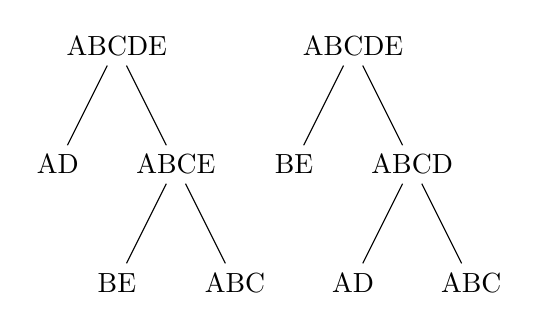
\begin{tikzpicture}
    \node (root1) at (0, 0) {ABCDE}
      child {node {AD}}
      child {node {ABCE}
        child {node {BE}}
        child {node {ABC}}};
    \node (root2) at (3, 0) {ABCDE}
      child {node {BE}}
      child {node {ABCD}
        child {node {AD}}
        child {node {ABC}}};
  \end{tikzpicture}
\end{figurebox}

Note that the decomposition that splits first $R[ABC]$ is not valid, since the resulting
relation $R[AB]$ is not a consequences of a functional dependency, see
\cref{fig:wrongdecomp}.

\begin{figurebox}[label=fig:wrongdecomp]{Invalid decomposition trees for the relation $R[ABCDE]$.}
  \centering
  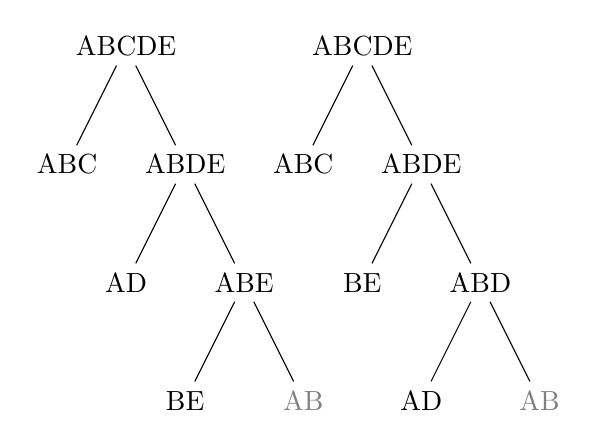
\begin{tikzpicture}
    \node (root1) at (0, 0) {ABCDE}
      child {node {ABC}}
      child {node {ABDE}
        child {node {AD}}
        child {node {ABE}
          child {node {BE}}
          child {node[gray] {AB}}}};
    \node (root2) at (3, 0) {ABCDE}
      child {node {ABC}}
      child {node {ABDE}
        child {node {BE}}
        child {node {ABD}
          child {node {AD}}
          child {node[gray] {AB}}}};
  \end{tikzpicture}
  \tcblower
  We consider the functional dependencies $A \to D$, $B \to E$, and $AB \to C$.
  Note that $R[AB]$ is not a consequence of a functional dependency.
\end{figurebox}

In this kind of relation schema, we have a set of key attributes, here $\mathcal{K} = AB$,
and a set of non-prime attributes, here $\mathcal{N} = CDE$.  Note that the case
$\mathcal{K} \cap \mathcal{N} = \emptyset$ is the simplest we can have.

Observe, however, that transitive dependencies\footnote{Actually, when an attribute is
both key and non-prime, some joins may generate invalid tables.} and complex join
dependencies restrict even further the joins we are allowed to perform.
% \textcolor{red}{Further formalization and study is under progress.}

Now, consider a very common case: in our dataset, keys are unknown.  Let $A$ be a student
id, $B$ be the course id, $D$ be the student age, $E$ be the course load, and $C$ be the
student grade at the course.  If only $CDE$ is known, the table $R[CDE]$ is already tidy
--- and the observational unit is the enrollment --- once there is no key to perform any
kind of normalization.  This happens in many cases where privacy is a concern.

But we can also consider that the observational unit is the student.  In this case, we
must perform joins traversing the leftmost decomposition tree in \cref{fig:decomp} from
bottom to top.  After each join, a summarization operation is performed on the relation
considering the student as the observational unit, i.e. over attribute $A$.  The first
join results in relation $R[ABCE]$ and the summarization operation results in a new
relation $R[AFG]$ where $F$ is the average grade and $G$ is the total course load taken by
the student.  They all calculated based on the rows that are grouped in function of $A$.
It is important to notice that, after the summarization operation, all observations must
contain a different value of $A$.  The second join results in relation $R[ADFG] = R[AD]
\bowtie R[AFG]$.  This relation has functional dependency $A \to DFG$, and it is in 3NF
(which is also tidy).

Unfortunately, it is not trivial to calculate all possible decomposition trees for a given
dataset.  It is up to the data scientist to decide which directions to follow.  However,
it is important to notice that the order of the joins and summarization operations are
crucial to the final result.
%\textcolor{red}{Further formalization and study is under progress.}

\subsection{Data semantics and interpretation}

In the rest of the book, we focus on a statistical view of the data.  Besides the
functional dependencies, we also consider the statistical dependencies of data.  For
instance, attributes $A$ and $B$ might not be functionally dependent, but they might exits
unknown $P(A, B)$ that we can estimate from the data.  Each observed value of a key can
represent a instance of a random variable, and the other attributes can represent
measured attributes or calculated properties.

For data analysis, it is very important to understand the relationships between the
observations.  For example, we might want to know if the observations are independent, if
they are identically distributed, or if there is a known selection bias.  We might also
want to know if the observations are dependent on time, and if there are hidden variables
that affect the observations.

Following wrong assumptions can lead to wrong conclusions.  For example, if we assume that
the observations are independent, but they are not, we might underestimate the variance of
the estimators.

Although we do not focus on time series, we must consider the temporal dependence of the
observations.  For example, we might want to know how the observation $x_t$ is affected by
$x_{t-1}$, $x_{t-2}$, and so on.  We might also want to know if Markov property holds,
and if there is periodicity and seasonality in the data.

For the sake of the scope of this book, we suggest that any prediction on temporal data
should be done in the state space, where it is safer to assume that observations are
independent and identically distributed.  This is a common practice in reinforcement
learning and deep learning. Takens' theorem\footfullcite{Takens1980} allows you to
reconstruct the state space of a dynamical system using time-delay embedding. Given a
single observed time series, you can create a multidimensional representation of the
underlying dynamical system by embedding the time series in a higher-dimensional space.
This embedding can reveal the underlying dynamics and structure of the system.

\section{Unstructured data}

Unstructured data are data that do not have a predefined data model or are not organized
in a predefined manner.  For example, text, images, and videos are unstructured data.

Every unstructured dataset can be converted into a structured dataset.  However, the
conversion process is not always straightforward nor lossless.  For example, we can
convert a text into a structured dataset by counting the number of occurrences of each
word.  However, we lose the order of the words in the text.

The study of unstructured data is, for the moment, out of the scope of this book.
